%% Figure 6 (pgfplots): Publication-grade grouped bar chart for Stateless Block-RMS saddle escape & Automata/LLM transfer.
\definecolor{stepc}{HTML}{0072B2}
\definecolor{outc}{HTML}{D55E00}
\definecolor{rmsc}{HTML}{009E73}
\definecolor{mutedc}{HTML}{6E6E6E}
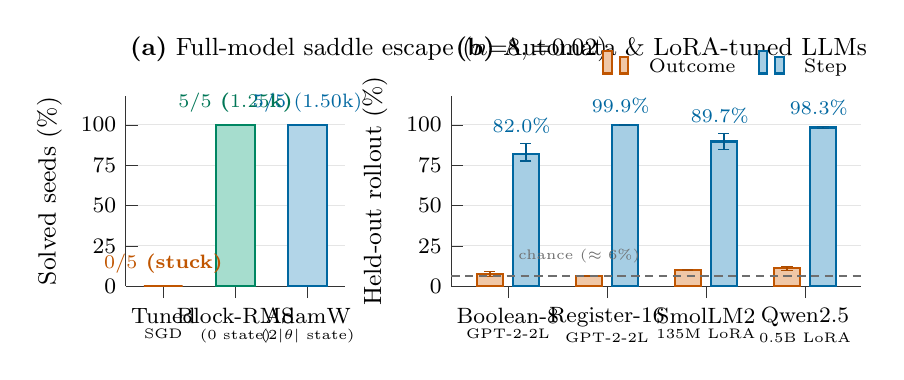
\begin{tikzpicture}
\pgfplotsset{
  every axis/.style={
    clip=false,
    height=4.0cm,
    ybar=3.5pt,
    ymin=0, ymax=118,
    ytick={0,25,50,75,100},
    axis line style={black!80},
    tick style={black!80},
    tick label style={font=\footnotesize},
    label style={font=\small},
    title style={font=\small, at={(0,1.04)}, anchor=south west, xshift=-2pt},
    axis x line*=bottom,
    axis y line*=left,
    ymajorgrids,
    major grid style={black!10}
  }
}

% Panel (a): Full-model optimizer saddle escape (n=8, p=1/4, d_model=64, eps=0.02)
\begin{axis}[
  name=pa,
  width=0.36\linewidth,
  bar width=14pt,
  ybar=0pt,
  bar shift=0pt,
  title={\textbf{(a)} Full-model saddle escape ($n{=}8, \initscale{=}0.02$)},
  ylabel={Solved seeds (\%)},
  symbolic x coords={Tuned SGD,Block-RMS,AdamW},
  xtick={Tuned SGD,Block-RMS,AdamW},
  xticklabels={{\shortstack{Tuned\\[-1pt]{\tiny SGD}}},{\shortstack{Block-RMS\\[-1pt]{\tiny ($0$ state)}}},{\shortstack{AdamW\\[-1pt]{\tiny ($2|\theta|$ state)}}}},
  enlarge x limits=0.26
]
  \addplot[draw=outc!90!black, fill=outc!25, line width=0.8pt] coordinates {(Tuned SGD,0)};
  \addplot[draw=rmsc!85!black, fill=rmsc!35, line width=0.9pt] coordinates {(Block-RMS,100)};
  \addplot[draw=stepc!90!black, fill=stepc!30, line width=0.8pt] coordinates {(AdamW,100)};

  \node[anchor=south, font=\scriptsize\bfseries, text=outc!90!black] at (axis cs:Tuned SGD,2) {$0/5$ (stuck)};
  \node[anchor=south, font=\scriptsize\bfseries, text=rmsc!75!black] at (axis cs:Block-RMS,101.5) {$5/5$ ($1.25$k)};
  \node[anchor=south, font=\scriptsize, text=stepc!90!black] at (axis cs:AdamW,101.5) {$5/5$ ($1.50$k)};
\end{axis}

% Panel (b): Multi-gate automata & Pretrained LLMs (Outcome vs Step)
\begin{axis}[
  name=pb,
  at={(pa.east)},
  anchor=west,
  xshift=1.35cm,
  width=0.56\linewidth,
  bar width=9.5pt,
  enlarge x limits=0.19,
  title={\textbf{(b)} Automata \& LoRA-tuned LLMs},
  ylabel={Held-out rollout (\%)},
  symbolic x coords={Boolean-8,Register-16,SmolLM2,Qwen2.5},
  xtick={Boolean-8,Register-16,SmolLM2,Qwen2.5},
  xticklabels={{\shortstack{Boolean-8\\[-1pt]{\tiny GPT-2-2L}}},{\shortstack{Register-16\\[-1pt]{\tiny GPT-2-2L}}},{\shortstack{SmolLM2\\[-1pt]{\tiny 135M LoRA}}},{\shortstack{Qwen2.5\\[-1pt]{\tiny 0.5B LoRA}}}},
  legend style={at={(1.0,1.04)}, anchor=south east, draw=none, fill=none, font=\scriptsize, legend columns=2, column sep=5pt, /tikz/every even column/.append style={column sep=6pt}}
]
  % Outcome bars
  \addplot[draw=outc!90!black, fill=outc!35, line width=0.8pt,
    error bars/.cd, y dir=both, y explicit, error bar style={outc!80!black, line width=0.8pt}]
    coordinates {
      (Boolean-8,7.7) += (0,1.2) -= (0,1.4)
      (Register-16,6.3) += (0,0.1) -= (0,0.1)
      (SmolLM2,9.9) += (0,0.2) -= (0,0.2)
      (Qwen2.5,11.1) += (0,1.2) -= (0,1.1)
    };
  % Step bars
  \addplot[draw=stepc!90!black, fill=stepc!35, line width=0.8pt,
    error bars/.cd, y dir=both, y explicit, error bar style={stepc!80!black, line width=0.8pt}]
    coordinates {
      (Boolean-8,82.0) += (0,6.2) -= (0,4.4)
      (Register-16,99.9) += (0,0.1) -= (0,0.1)
      (SmolLM2,89.7) += (0,4.9) -= (0,4.9)
      (Qwen2.5,98.3) += (0,0.7) -= (0,0.8)
    };
  \legend{Outcome, Step}

  % Chance dashed line
  \draw[mutedc, densely dashed, line width=0.75pt] (rel axis cs:0,0.053) -- (rel axis cs:1,0.053);
  \node[anchor=south, font=\tiny, text=mutedc, xshift=-10pt] at (axis cs:Register-16,8.5) {chance ($\approx 6\%$)};

  % Value annotations above Step bars
  \node[anchor=south, font=\scriptsize\bfseries, text=stepc!90!black, xshift=5pt] at (axis cs:Boolean-8,88.5) {$82.0\%$};
  \node[anchor=south, font=\scriptsize\bfseries, text=stepc!90!black, xshift=5pt] at (axis cs:Register-16,101.0) {$99.9\%$};
  \node[anchor=south, font=\scriptsize\bfseries, text=stepc!90!black, xshift=5pt] at (axis cs:SmolLM2,95.0) {$89.7\%$};
  \node[anchor=south, font=\scriptsize\bfseries, text=stepc!90!black, xshift=5pt] at (axis cs:Qwen2.5,99.5) {$98.3\%$};
\end{axis}
\end{tikzpicture}
